
\documentclass[titlepage,a4paper]{article}

\usepackage{a4wide}
\usepackage[colorlinks=true,linkcolor=black,urlcolor=blue,bookmarksopen=true]{hyperref}
\usepackage{bookmark}
\usepackage{fancyhdr}
\usepackage[spanish]{babel}
\usepackage[utf8]{inputenc}
\usepackage[T1]{fontenc}
\usepackage{graphicx}
\usepackage{float}
\usepackage{listings}
\usepackage{color}

\pagestyle{fancy} % Encabezado y pie de página
\fancyhf{}
\fancyhead[R]{Algoritmos y Programación III - FIUBA}
\renewcommand{\headrulewidth}{0.4pt}
\fancyfoot[C]{\thepage}
\renewcommand{\footrulewidth}{0.4pt}

\begin{document}
\begin{titlepage} % Carátula
	\hfill\includegraphics[width=6cm]{logofiuba.jpg}
    \centering
    \vfill
    \Huge \textbf{Trabajo Práctico 2 — Java}
    \vskip2cm
    \Large [7507/9502] Algoritmos y Programación III\\
    Curso 1 \\ % Curso 1 para el de la tarde y 2 para el de la noche
    Grupo 14 \\
    Primer cuatrimestre de 2020
    \vfill
    Integrantes\\[1\baselineskip]

    Baffetti Mariano\\
    Cuppari Juan\\
    Hoszowski Juan\\
    Iskandarani Roberto\\
    Perez Ignacio\\
    \vfill
    Corrector: Edson Justo
    \vfill
\end{titlepage}

\tableofcontents % Índice general
\newpage

\section{Introducción}\label{sec:intro}
El presente informe reune la documentación de la solución del segundo trabajo práctico de la materia Algoritmos y Programación III que consiste en desarrollar un juego de preguntas y respuestas, denominado Kahoot, en Java utilizando los conceptos del paradigma de la orientación a objetos vistos hasta en el curso. En el juego participan al menos dos jugadores, que deben ir respondiendo por turnos. Las preguntas pueden ser de distinto tipo (Verdadero o falso, Multiple Choice, Ordered Choice, Group Choice) y además pueden tener bonificaciones asociadas (X2, X3, exclusividad de puntaje). Al finalizar el juego se indica quien ha sido el jugador que obtuvo el mayor puntaje.


\section{Supuestos}\label{sec:supuestos}
\begin{itemize}
    \item El tiempo para cada turno es de 30 segundos.
\end{itemize}
\begin{itemize}
    \item Un jugador puede tener puntaje negativo, esto se da debido a las preguntas con penalidad ya que por cada opción incorrecta se le resta un punto.
\end{itemize}
\begin{itemize}
    \item En caso de tener el mismo puntaje, puede haber más de un ganador.
\end{itemize}
\begin{itemize}
    \item No pueden haber dos jugadores con el mismo nombre.
\end{itemize}
\begin{itemize}
    \item En las preguntas de tipo Ordered Choice y Group Choice la respuesta se considera correcta siempre que todas las opciones seleccionadas sean correctas.
\end{itemize}
\begin{itemize}
    \item En las preguntas de tipo Ordered Choice y Group Choice se suma un punto por cada opción correcta en caso de que la respuesta sea correcta.
\end{itemize}


\section{Diagramas de Clases}\label{sec:diagramasdeclases}
% Mostrar las secuencias interesantes que hayan implementado. Pueden agregar texto para explicar si algo no queda claro.

\begin{figure}[H]
\centering
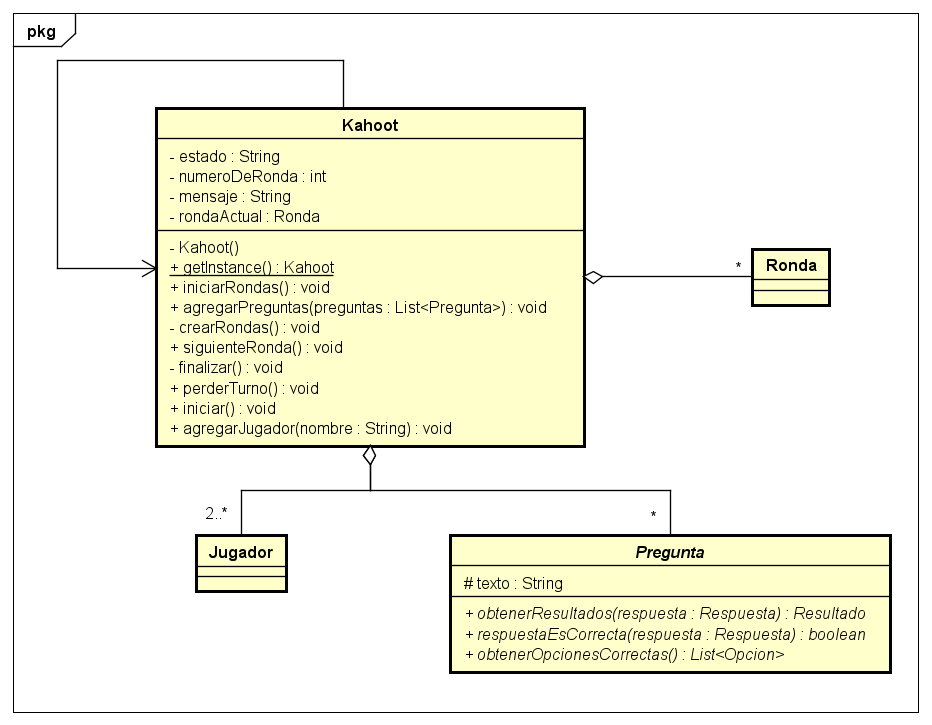
\includegraphics[width=1.1\textwidth]{Diagrama de clases Kahoot.png}
\caption{\label{fig:seq01}Diagrama general de la aplicación.}
\end{figure}

\begin{figure}[H]
\centering
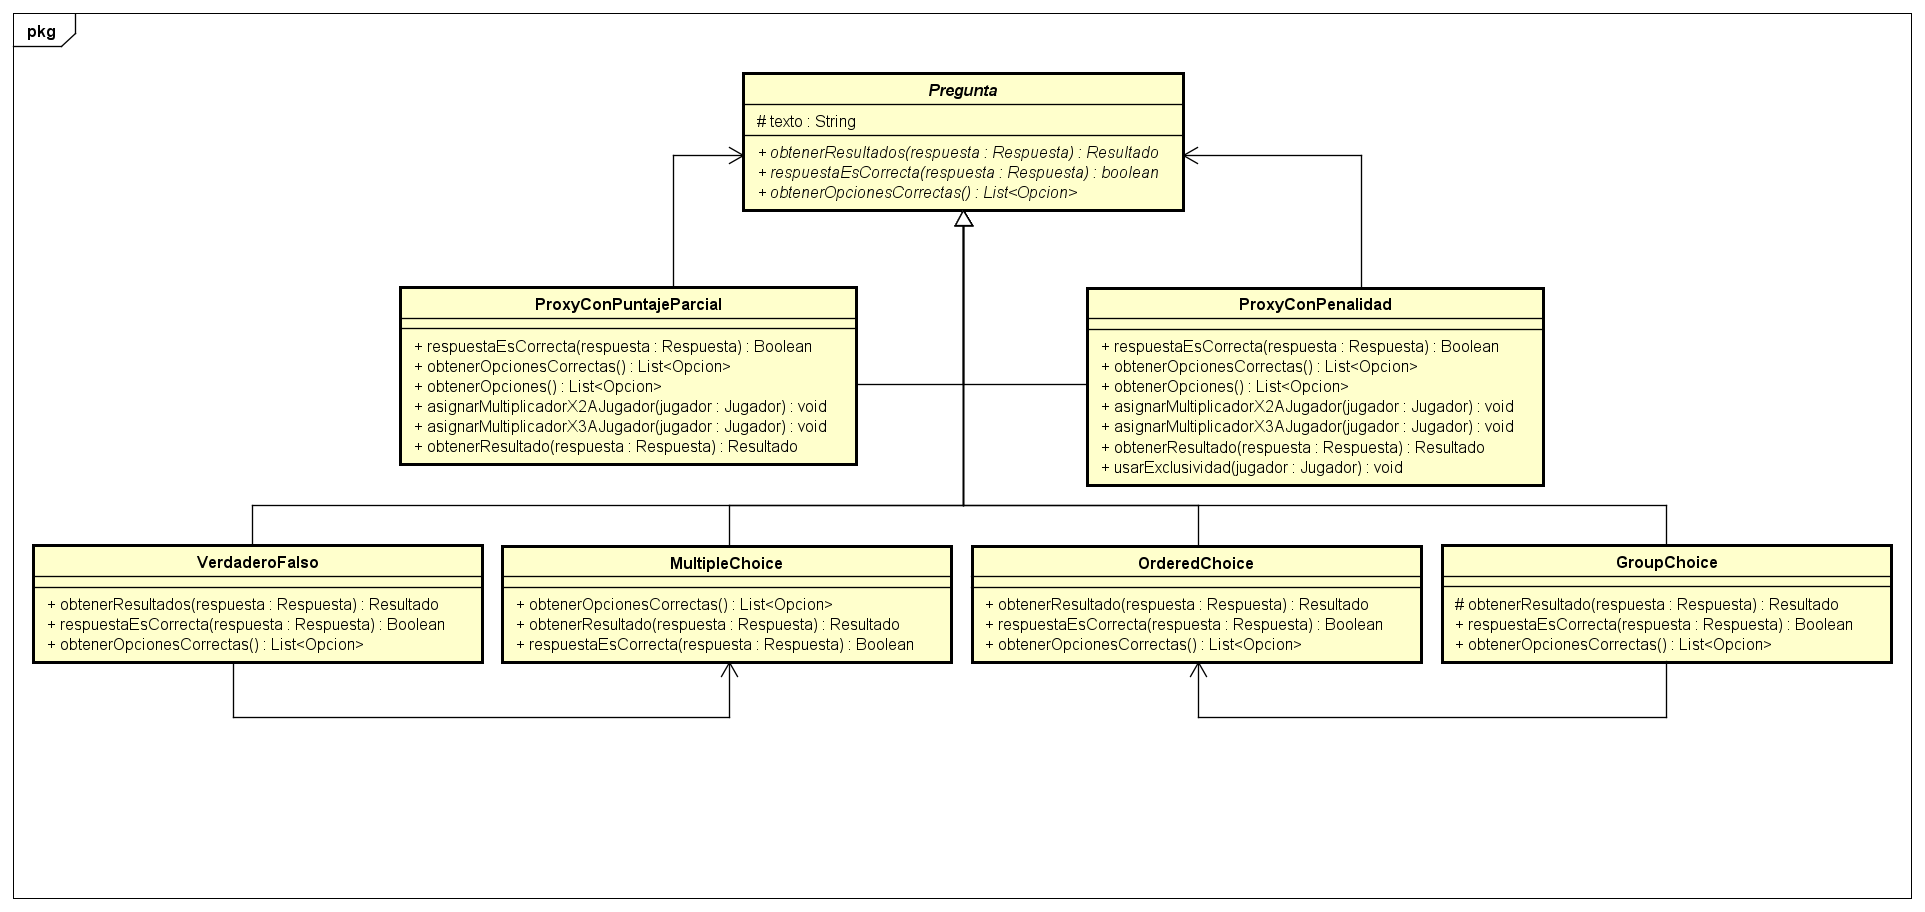
\includegraphics[width=1.1\textwidth]{Diagrama de clases Pregunta.png}
\caption{\label{fig:seq01}Diagrama de preguntas.}
\end{figure}

\begin{figure}[H]
\centering
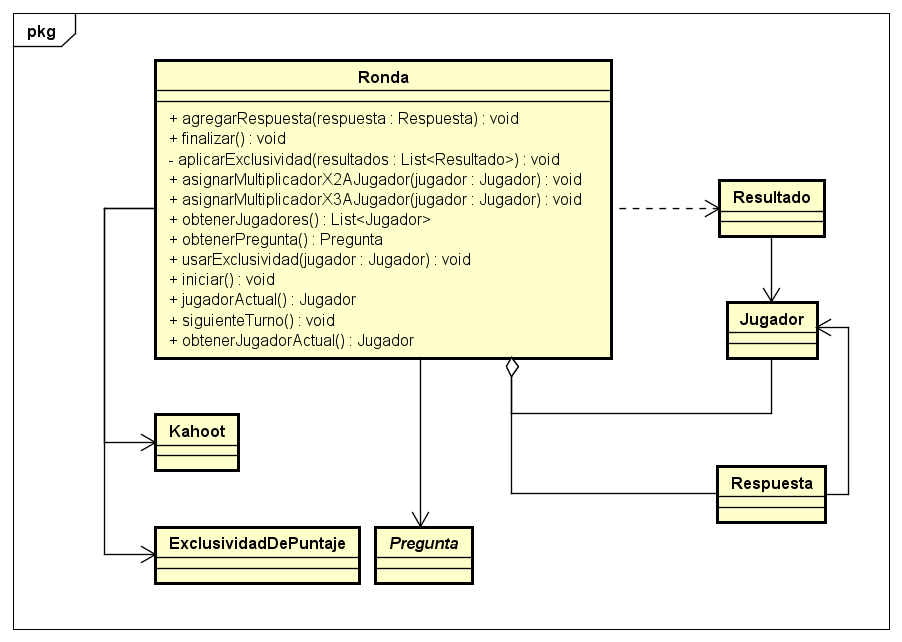
\includegraphics[width=1.1\textwidth]{Diagrama de clase Ronda.png}
\caption{\label{fig:seq01}Diagrama de Ronda.}
\end{figure}


\section{Diagramas de secuencia}\label{sec:diagramasdesecuencia}
% Mostrar las secuencias interesantes que hayan implementado. Pueden agregar texto para explicar si algo no queda claro.

\begin{figure}[H]
\centering
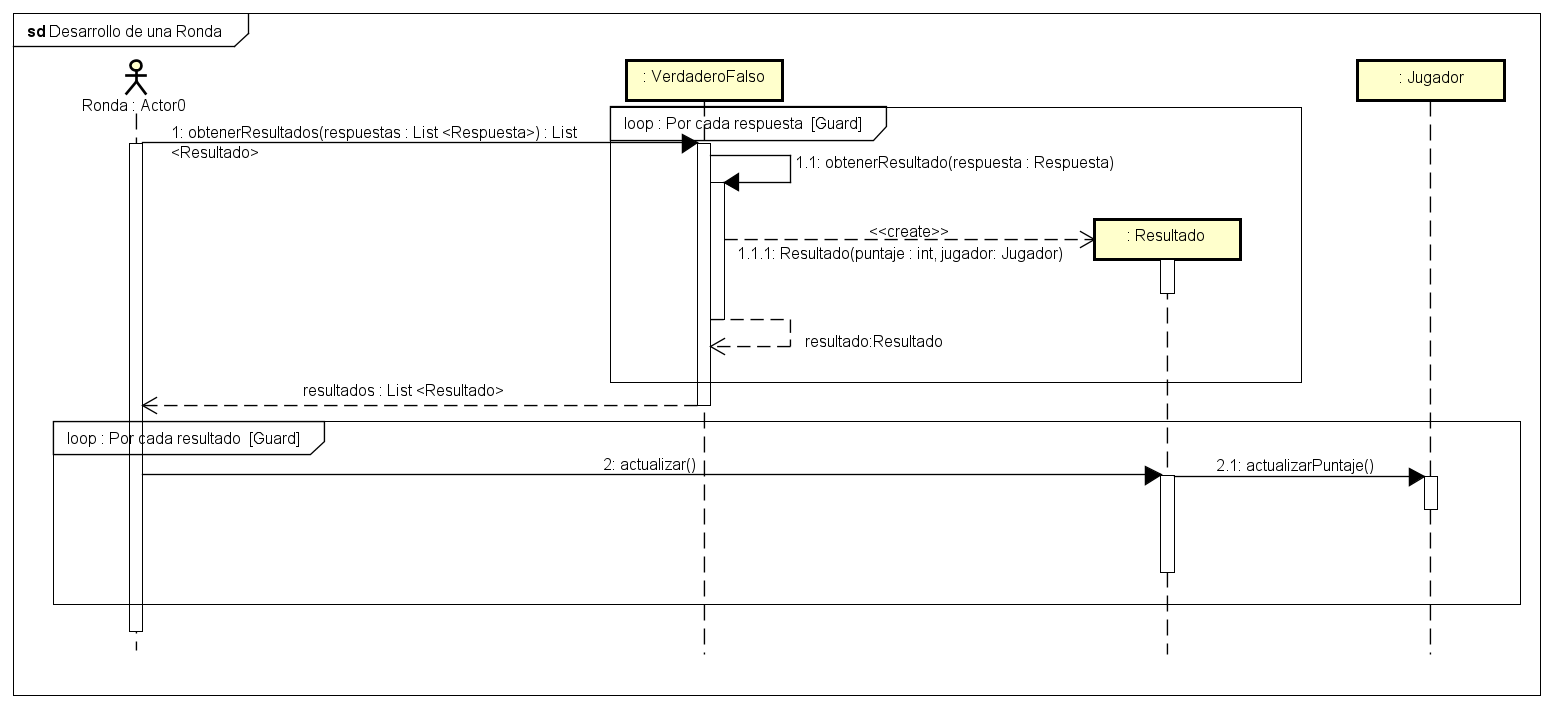
\includegraphics[width=1.1\textwidth]{Desarrollo de una Ronda.png}
\caption{\label{fig:seq01}Desarrollo de una ronda.}
\end{figure}

\begin{figure}[H]
\centering
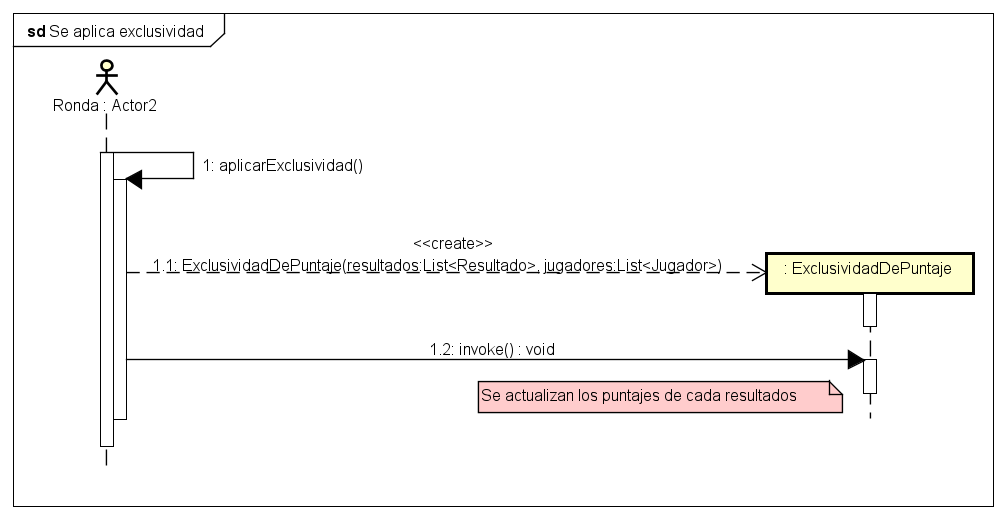
\includegraphics[width=1.1\textwidth]{Se aplica exclusividad.png}
\caption{\label{fig:seq01}Se aplica exclusividad.}
\end{figure}

\begin{figure}[H]
\centering
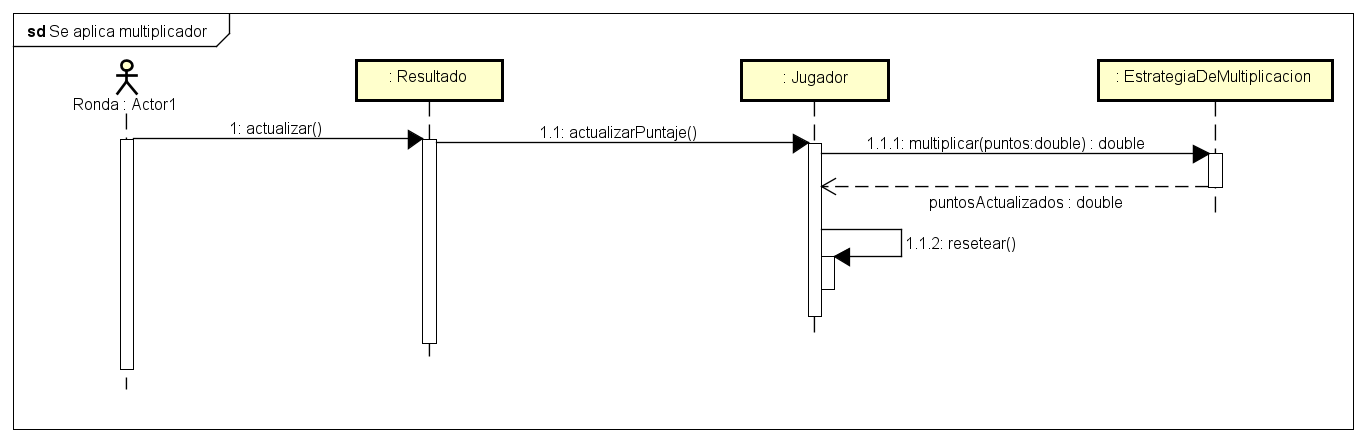
\includegraphics[width=1.1\textwidth]{Se aplica multiplicador.png}
\caption{\label{fig:seq01}Se aplica multiplicador.}
\end{figure}

\begin{figure}[H]
\centering
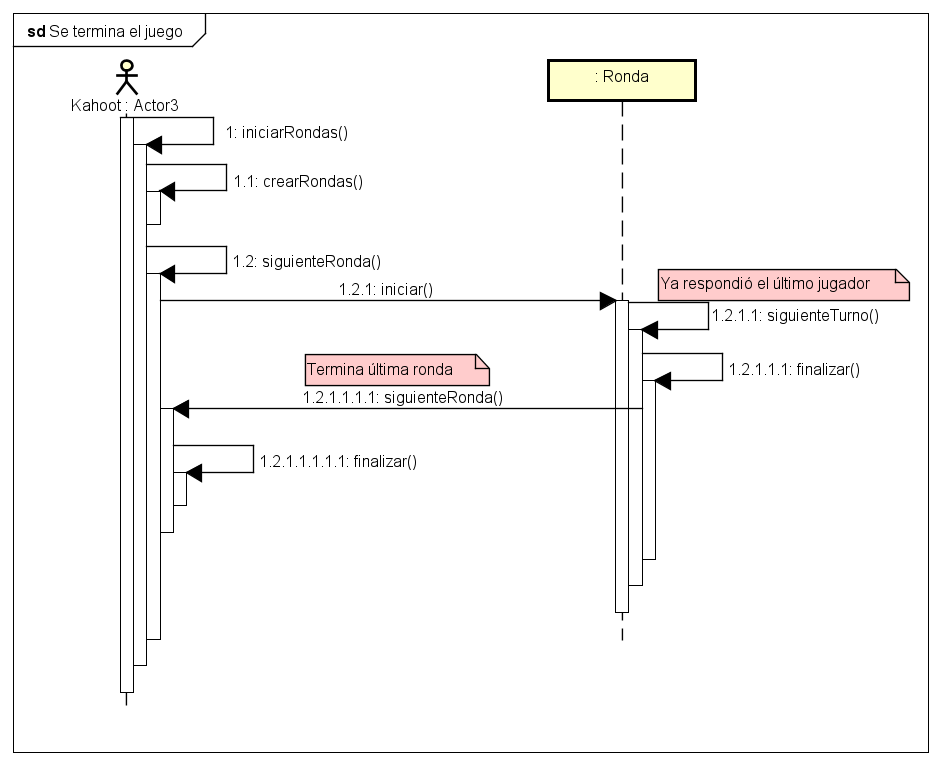
\includegraphics[width=1.1\textwidth]{Se termina el juego.png}
\caption{\label{fig:seq01}Se termina el juego.}
\end{figure}

\section{Diagramas de Paquetes}\label{sec:diagramasdepaquetes}

\begin{figure}[H]
\centering
\includegraphics[width=1.1\textwidth]{sequence-diagram-1.png}
\caption{\label{fig:seq01}Responder una pregunta y asignar puntos.}
\end{figure}


\section{Diagrama de Estado}\label{sec:diagramasdeestado}

\begin{figure}[H]
\centering
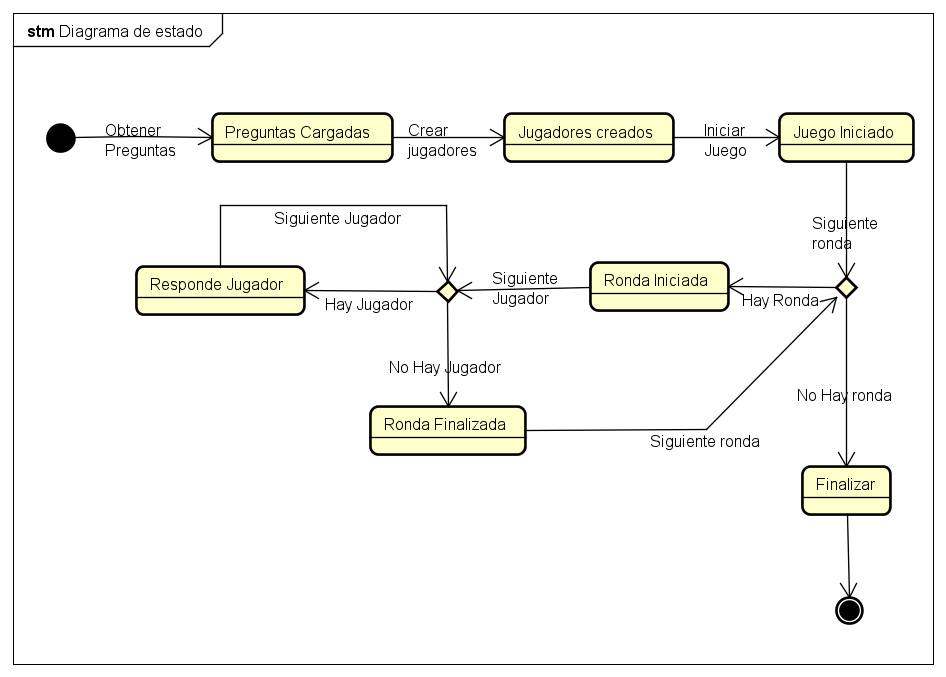
\includegraphics[width=1.1\textwidth]{Diagrama de estado.png}
\caption{\label{fig:seq01}Diagrama de estados del juego.}
\end{figure}

\section{Diagrama de Paquetes}\label{sec:diagramasdepaquete}

\begin{figure}[H]
\centering
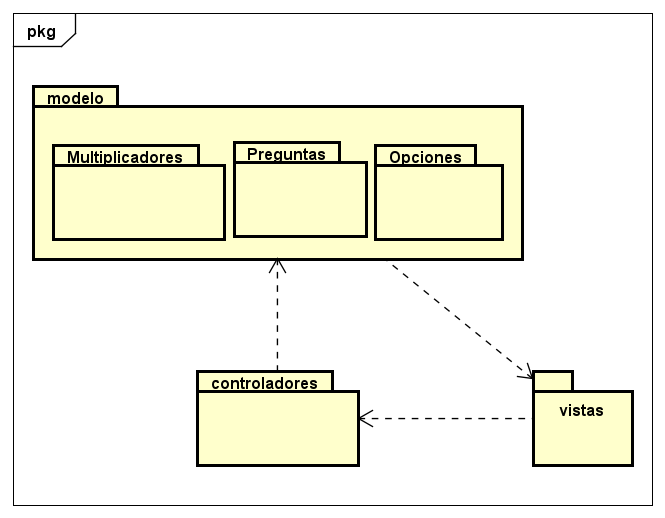
\includegraphics[width=1.1\textwidth]{Diagrama de Paquetes.png}
\caption{\label{fig:seq01}Diagrama de paquetes de la aplicación.}
\end{figure}


\section{Detalles de Implementación}\label{sec:detallesdeimplementacion}

\subsection{Penalidad, Puntaje Parcial, Multiplicadores y Exclusividad} Se utilzó el patrón proxy para poder modificar el comportamiento de las preguntas y hacer que se comporten como preguntas con penalidad o con puntaje parcial. Por ejemplo, si se necesita crear una pregunta Verdadero o Falso con penalidad, se crea una pregunta de tipo ProxyConPenalidad, la cual tiene una referencia a una instancia de verdadero o falso. De
ésta manera, no solamente se puede agregar éste comportamiento a los nuevos tipos de pregunta que vayan surgiendo, sino que también los proxies sirven para controlar el uso de Multiplicadores y Exclusividad. Se evaluó como alternativa el uso del patrón decorator, que permite modificar el comportamiento de la clase en tiempo de ejecución. En nuestro caso, sólo necesitabamos tener flexibilidad en tiempo de diseño.

\subsection{Multiplicadores} Se utilizó el patrón Strategy para la implementación de multiplicadores. Al realizar el calculo de puntajes, el jugador le pide al multiplicador en uso (por defecto hay un multiplicador que sólo multiplica x1) que multiplique su puntaje. Otro detalle importante de ésta implementación, es que los jugadores se instancian con una lista de multiplicadores de la cual se van eliminando los que el jugador vaya utilizando. Una ventaja de \’este enfoque es que permite que al jugador se le agreguen o quiten multiplicadores una vez que el juego haya empazado.

\subsection{Implementación de Kahoot} Se utilizó el patrón Singletón para la implementación de la clase Kahoot. Ésta clase es a su vez un Facade, que permite a los controladores modificar el estado del modelo.
\subsection{Implementación de MVC} Se utilizó el patrón Observer para la implementación del patrón MVC. La clase Kahoot es un Observable que es observado por KahootVista. Todas las vistas que tienen controles que permitan modificar el modelo, tienen una referencia a un controlador (a veces específico) que les permite interactuar con el modelo.
\subsection{Exclusividad de puntaje} La exclusividad de puntaje se calcula al final de cada ronda, y para su cálculo es necesario conocer a todas las respuestas y a los jugadores que formaron parte de la ronda. Para evitar dejar la responabilidad del cálculo en la clase Ronda, se creó un objeto ExclusividadDePuntaje (method object) cuya única responsabilidad es realizar ese cálculo.
\subsection{Vistas de Preguntas} Para seleccionar el tipo de vista de pregunta que se debe instanciar se utilizó el patrón Factory Method. La clase FactoryPreguntasVista tiene un hash como atributo, que contiene como clave un String que permite identificar a la clase y como valor a la clase de la pregunta que se debe instanciar (Ej: VerdaderoOFalsoVista.class). De ésta forma se puede instanciar la clase en particular de forma dinamica.
\begin{lstlisting}[language=java]
    public Pane crear(String tipoPregunta, Kahoot kahoot) {
        Class<?> clase = this.vistas.get(tipoPregunta);
        Pane vista = null;

        try {
            vista = (Pane) clase.getDeclaredConstructor(Kahoot.class).newInstance(kahoot);
        } catch (InstantiationException e) {
            e.printStackTrace();
        } catch (IllegalAccessException e) {
            e.printStackTrace();
        } catch (InvocationTargetException e) {
            e.printStackTrace();
        } catch (NoSuchMethodException e) {
            e.printStackTrace();
        }

        return vista;
    }

\end{lstlisting}

\subsection{Creación de preguntas} Se utilizó una combinación de patrón builder con fluent api para la creación de preguntas. Por ejemplo, para la creación de una pregunta VerdaderoOFalso con penalidad se utiliza la siguiente sintaxis:
\begin{lstlisting}[language=java]
    var builder = new PreguntasBuilder();
    var pregunta = builder
                .crearVerdaderOFalso("texto de pregunta", opciones)
                .conPenalidad()
                .get();
\end{lstlisting}




\section{Excepciones}\label{sec:excepciones}

\begin{description}
\item[YaHayUnMultiplicadorEnUsoError:] Excepción que se lanza cuando un jugador intenta usar más de un multiplicador en un mismo turno, mostrando un cartel de advertencia.

\end{description}

\begin{description}
\item[YaHayUnaExclusividadEnUsoError:] Excepción que se lanza cuando un jugador intenta usar más de un bonificador de exclusividad en un mismo turno, mostrando un cartel de advertencia.

\end{description}

\begin{description}
\item[YaExisteJugadorConEseNombreError:] Excepción que se lanza cuando un jugador intenta registrarse con un nombre ya utilizado, mostrando un cartel de advertencia para que modifique el nombre ingresado.

\end{description}

\begin{description}
\item[NoSePuedeUtilizarMultiplicadorError:] Excepción que se lanza cuando un jugador intenta utilizar un multiplicador en una pregunta que no permite el uso del mismo.

\end{description}

\begin{description}
\item[NoSePuedeUtilizarExclusividadError:] Excepción que se lanza cuando un jugador intenta utilizar un bonificador de exclusividad en una pregunta que no permite el uso del mismo.

\end{description}

\begin{description}
\item[NoSePuedeIniciarJuegoSiNoHayPreguntasError:] Excepción que se lanza cuando el programa no detecta ninguna pregunta cargada.

\end{description}

\begin{description}
\item[NoSePuedeIniciarJuegoSiNoHayJugadoresError:] Excepción que se lanza cuando se intenta iniciar el juego sin tener ningún jugador registrado.

\end{description}

\begin{description}
\item[NoSeEncuentraElMultiplicadorError:] Excepción que se lanza cuando un jugador intenta utilizar un multiplicador cuando ya se agotaron, mostrando un cartel de advertencia.

\end{description}

\begin{description}
\item[NoHayExclusividadesDisponiblesError:] Excepción que se lanza cuando un jugador intenta utilizar un bonificador de exclusividad cuando ya se agotaron, mostrando un cartel de advertencia.

\end{description}

\begin{description}
\item[JugadorNoSePuedeCrearConNombreVacioError:] Excepción que se lanza cuando se intenta registrar un jugador sin haber ingresado ningún caracter, mostrando un cartel de advertencia.

\end{description}


\end{document}